% subsection of GoTxn proof section
\subsection{Lifting specification for journaling (\scc{jrnl})}
\label{sec:txn:lifting}

Lifting is defined at an intermediate layer, \scc{jrnl} (for journaling), rather
than for \scc{txn} which is the top-level API of GoTxn. Journaling uses what we
call ``operations'' to distinguish them from ``transactions'' --- reads and
writes are performed from within the context of an operation, and like a
transaction the writes are committed atomically to
disk, but the difference is that the calling library is responsible for guaranteeing
concurrent operations manipulate disjoint sets of addresses. The complete API is
shown in \cref{fig:jrnl-api}. In the case of GoTxn, that caller is
the two-phase locking code, whose proof is described in \cref{sec:txn:refinement}.

\begin{figure}[ht]
  \begin{minted}{go}
func Begin() *Op
func (op *Op) Commit()

func (op *Op) Read(a Addr, szBits uint64) []byte
func (op *Op) Write(a Addr, szBits uint64, d []byte)
  \end{minted}
  \tightenspace
  \caption[API for the journaling layer.]{The API for the journaling layer, \scc{jrnl}. There is no
    \cc{Abort()} method (the caller simply abandons the \cc{op} struct). Reads
    and writes support bit-sized objects within the same API.\@ The \cc{Addr}
    struct is the same as one given in the GoTxn API (\cref{fig:txn-api}).}
  \label{fig:jrnl-api}
\end{figure}

In the lifting specification, there is a global, logical disk representing the
state of the journaling system, and within each ongoing operation there is an
operation-local view of the disk. The operation-local view is like the disk
view but also incorporates buffered writes. The durable views are disjoint, so
that an address is either in the global disk or ``lifted'' into a particular
operation. Disjointness is what guarantees that every operation-local view is really local and
doesn't change due to concurrent threads.

The lifting-based specification uses a logical concept of ownership to keep all
of these views disjoint and consistent. The state of each view is defined using ghost state
in Iris, and the proof uses separation-logic resources to express ownership over that
ghost state; for a general introduction to the idea of
ownership in separation logic, see \cref{sec:perennial:concurrency}. The
journaling proof issues three types of resources, all per-address:
$a \mapstoDisk o$, $a \mapstoOp o$, and $a \mapstoLftd o$. The first is the most
straightforward: $a \mapstoDisk o$ asserts that the global durable disk has
value $o$ at address $a$ (we use the metavariable $o$ since these addresses have
objects that can be smaller than a block, such as a 128-byte inode value or even
a single bit). In addition, $a \mapstoDisk o$ expresses ownership over the
address $a$. The second resource, $a \mapstoOp o$, asserts ownership of the
operation-local view associated with an in-memory operation $\mathit{op}$; it
mean that either the on-disk value is $o$ or that $\mathit{op}$ contains a
buffered write with the value $o$ to address $a$. The last resource,
$a \mapstoLftd o$ is similar to $a \mapstoDisk o$, but the difference is related
to lifting and explained below.

The life cycle of these resources, as they are modified by lifting, writes,
commit, and crashes, is shown in \cref{fig:gojournal-resources}. The complete
specifications are detailed in the remainder of this section.

\begin{figure}[hb]
  \centering
  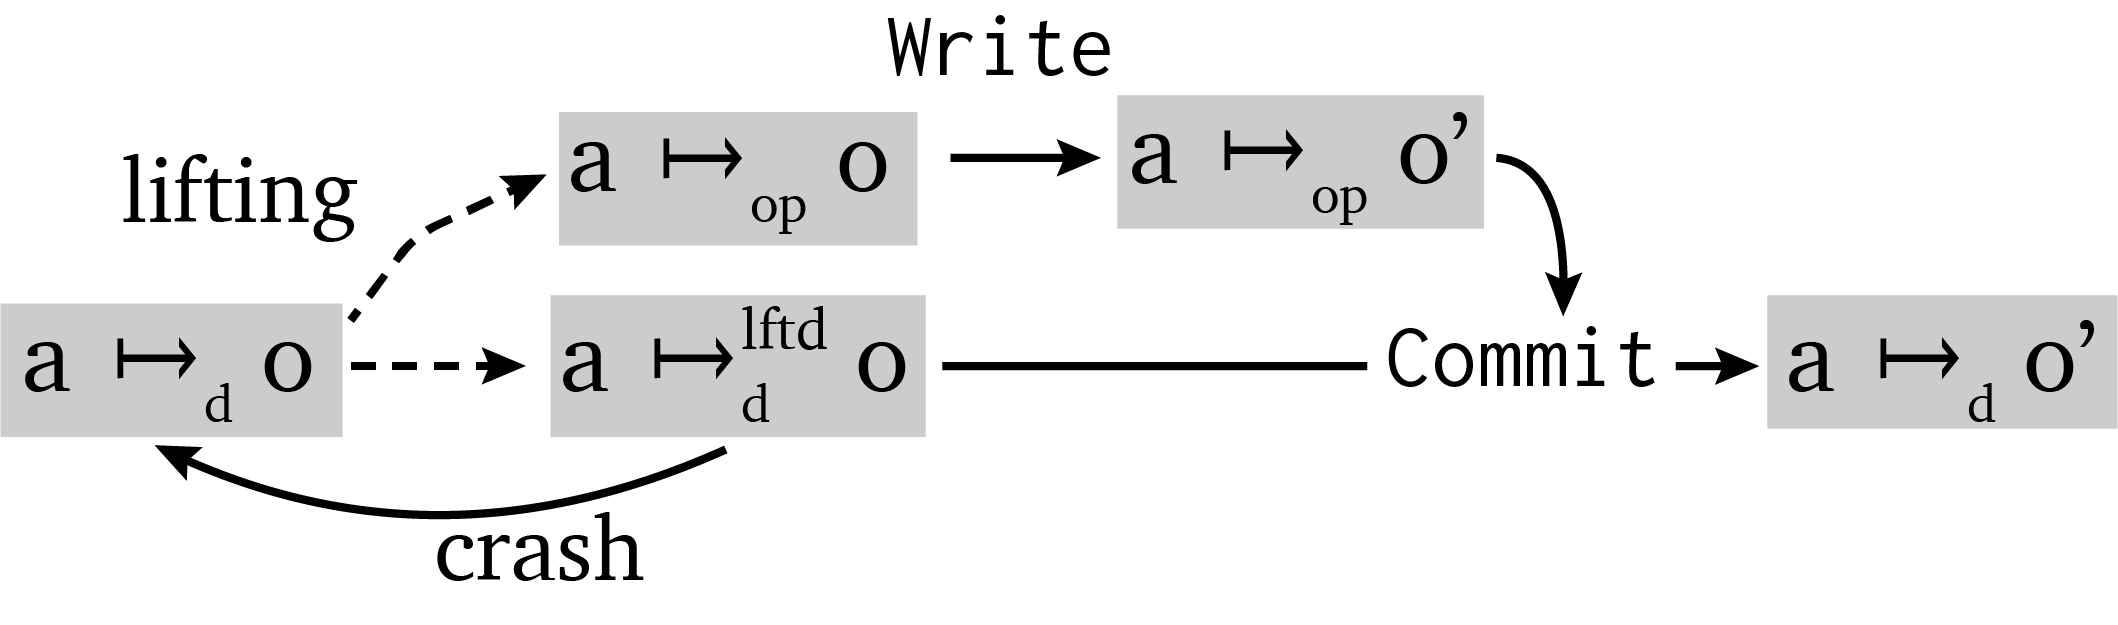
\includegraphics{fig/gojournal-resources.png}
  \caption{Life cycle for the resources in the lifting specification.}
  \label{fig:gojournal-resources}
\end{figure}


\subsubsection{Initialization}

The first step in using the journaling specification is to initialize the whole
system. Initialization is somewhat complicated by restrictions GoTxn places
on how sub-block objects are used. The proof requires the caller to fix ahead of
time (when the whole journaling system is initialized) a size for
the objects within each block. Currently our proofs assume that objects are either a single bit, 128
bytes (to hold inodes), or a full block, but supporting an arbitrary
power-of-two-sized block should be a
straightforward extension. To initialize the system, the caller supplies a
``schema'' which gives a size for the objects in each disk offset (that is, every 4KB
aligned offset, not the journal's logical sub-block addresses); this enforces
that all the objects within a block are of the same size.

The journal's initialization is specified by giving the caller a lemma that
transform ownership over the entire physical disk into the precondition for the
journal's recovery procedure; from this point forward the usual crash and
recovery reasoning in Perennial applies. For each offset $i$ and block size $k$, the initial ownership for that disk
block consists of the address $(i, k \times o)$ within that block (this is
mathematical notation for the Go struct
\texttt{Addr\{Blkno:\;i, Offset:\;k*o\}}).
More formally the initial ownership for a given $i$ and $k$ is given by the
following definition:
\[
  \operatorname{zeroObjects}(i, k) \defeq \bigast_{0 \leq k \times o < 4096} (i, k \times o) \mapstoDisk 0
\]


The initialization lemma \ruleref{jrnl-init} creates resources
for all of these initial objects,
starting from an all-zero disk. The lemma takes a schema
$\mathit{kinds}$ that maps disk addresses to block sizes and a disk size $s$;
this schema is arbitrary but fixed at initialization time. We use
$i \mapsto_{\mathrm{disk}} 0$ to denote ownership over a physical disk offset $i$
(not to be confused by the $a \mapstoDisk o$ issued by the journaling proof).
\begin{mathpar}
  \inferH{jrnl-init}{}{
{\begin{aligned}
  &513 \leq s \land \dom(\mathit{kinds}) = \{ i \mid 513 \leq i < s \} \land {} \\
  &\bigast_{0 \leq i < s} i \mapsto_{\mathrm{disk}} 0 \wand {} \\
  &\vs \cc{is_txn_crash_condition}(\mathit{kinds}) \sep {} \\
  &\quad \bigast_{(i,k) \in \mathit{kinds}} \operatorname{zeroObjects}(i, k)
\end{aligned}}
}
\end{mathpar}

Notice that this initialization is just a logical operation; the schema is not
even required at runtime for the code. It creates \cc{is_txn_crash_condition},
which is the precondition and crash condition for the transaction system's
recovery procedure. The journal objects in this lemma's conclusion are initially
fully owned by recovery, which then shares them with threads. The journaling
system's proof does not fix a particular mechanism for \emph{how} access to these resources is mediated; it
simply requires exclusive access to an address in the form of a
$a \mapstoDisk o$ resource. In practice, GoTxn mediates access to
$a \mapstoDisk o$ by protecting it with a per-address lock.

\subsubsection{Preparing operations}

\newcommand{\isop}{\cc{is_op}(\mathit{op})}

The specification for \cc{Begin()} is straightforward, since the operation has
not yet interacted with the disk:
%
\begin{align*}
  \hoareV{\TRUE}%
  {\cc{Begin}()}%
  {\Ret{op} \isop}
\end{align*}
The specification has a trivial precondition of $\TRUE$ and its postcondition
returns an assertion \cc{is_op}, which says that $\mathit{op}$ is a valid
\cc{*Op} object that represents a journaling operation.  (This is different from
the \cc{*Txn} struct that represents an ongoing transaction, which has additional
state to track the locks acquired so far.) The operation starts out with an empty operation-local
view and ownership over no addresses; the ghost state for this operation's view
is initialized by the proof of this theorem and represented as part of
$\cc{is_op}(\mathit{op})$.

In order to interact with an address within an operation, the specification
requires the caller to start with $a \mapstoDisk o$ and then \emph{lift} it to
obtain an operation-local resource, where lifting is the following purely
logical operation \ruleref{jrnl-lift}:
\begin{mathpar}
  \inferH{jrnl-lift}{}{\isop \sep a \mapstoDisk o \vs \isop \sep a \mapstoOp o \sep a \mapstoLftd o}
\end{mathpar}

Notice that the result of lifting is both an operation-local assertion and
$a \mapstoLftd o$; this latter assertion is much like $a \mapstoDisk o$ in that
it asserts the on-disk value of address $a$, but it cannot be lifted again. This
is required for soundness; only one of $a \mapstoDisk o$ and $a \mapstoOp o$ is
allowed for ownership to actually be exclusive. Lifting takes and preserves
$\cc{is_op}(\opv)$, which reflects that the ghost state for $\opv$ has
been set up.

The specification for \cc{OverWrite} describes the effect of writing to the
local memory of a buffered journal operation:
%
\begin{align*}
  \hoareV{\isop \sep a \mapstoOp o \sep \cc{buf_obj}(buf, o')}%
        {\mathit{op}.\cc{OverWrite}(a, buf)}%
        {\isop \sep a \mapstoOp o'}
  %\tagH{OverWriteSpec}
\end{align*}

The precondition includes $\cc{buf_obj}(buf, o')$ to say that the in-memory
buffer $buf$ encodes the object to be written $o'$.
The \cc{is_op} predicate is both
required and returned by the specification, which reflects the fact that
\cc{OverWrite} operates on the in-memory and ghost state covered by
this predicate.

The specification for \cc{ReadBuf} is similar. \cc{ReadBuf}
returns a buffer that points into the \cc{op} struct, so it has a more
sophisticated spec:
%
\begin{align*}
  \hoareV{\isop \sep a \mapsto_{\mathit{op}} o}%
        {op.\cc{ReadBuf}(a)}%
        {\Ret{buf}
  \begin{aligned}
  &\cc{buf_obj}(\mathit{buf}, o) \sep \phantom{} \\
  &\quad( \cc{buf_obj}(\mathit{buf}, o) \wand \\
  &\quad\quad \isop \sep a \mapsto_{\mathit{op}} o )
    \end{aligned}}
    %\tagH{ReadBufSpec}
\end{align*}

This states that, when \cc{ReadBuf} finishes, it returns a buffer $\mathit{buf}$
and two resources: $\cc{buf_obj}(\mathit{buf}, o)$ says the buffer has the old
object $o$, while the second is a separating implication or \emph{wand} $\wand$.
The wand says that if
the caller returns ownership of $\cc{buf_obj}(\mathit{buf}, o)$, it can get back
the $\cc{is_op}(\mathit{op})$ predicate. This allows the caller to use the
buffer to read the data before continuing to read and write within the
operation. The complete specification in the \scc{jrnl} layer also supports modifying the
object using the buffer returned by \cc{ReadBuf}~\cite{chajed:gojournal}, but
GoTxn does not expose that feature.

\subsubsection{Commit}

The final method in the journaling API is \cc{Commit()}, which atomically
persists all the writes buffered in the operation. The specification is based on
two maps $m$ and $m'$ whose domains are the set of all addresses lifted into the
operation. The first map $m$ gives the on-disk, pre-operation values while $m'$
has the new values buffered in the operation.
\begin{align*}
  \hoareCV{ \begin{aligned}
              &\dom(m) = \dom(m') \sep {} \\
  &\left( \bigast_{(a,o) \in m} a \mapstoLftd o \right) \sep %
  \left( \bigast_{(a,o') \in m'} a \mapstoOp o' \right)
            \end{aligned}} %
  {\mathit{op}.\cc{Commit}()}%
  {\Ret{\mathit{ok}} \mathrm{if~} \mathit{ok} %
  \mathrm{~then~} \bigast_{(a,o') \in m'} a \mapstoDisk o' \mathrm{~else~} %
    \bigast_{(a,o) \in m} a \mapstoDisk o}%
  {\left( \bigast_{(a,o) \in m} a \mapstoDisk o \right) \lor
    \left( \bigast_{(a,o') \in m'} a \mapstoDisk o' \right) }
\end{align*}

The precondition in this specification requires ownership over a subset of the
logical disk, the addresses in $\dom(m)$, both on disk and within the
operation-local view. If the system does not crash and returns
$\mathit{ok} = \goosetrue$, \cc{Commit} returns ownership over the new values
on disk. It returns full disk points-to assertions $a \mapstoDisk o'$ because
these addresses are ``lowered'' so that subsequent operation can lift them
again. If the commit aborts (which only happens if the transaction does not fit
in memory), then the specification still returns full disk ownership albeit with
the old values. The crash condition of the \cc{Commit} specification captures
that even if the system crashes, it still returns ownership over the disk
resources, with either the old or new values. Whether this disjunction goes to
the left- or right-hand side depends on exactly when the system crashes; see
\cref{sec:perennial:recovery-spec} for a discussion of how the proof handles
this.

It's a little easier to see the overall structure of \cc{Commit}'s specification
when specialized to a single address (although the real specification is powerful
precisely because it captures atomicity across multiple addresses):
\begin{align*}
  \hoareCV{a \mapstoLftd o \sep a \mapstoOp o'} %
  {\mathit{op}.\cc{Commit}()}%
  {\Ret{\mathit{ok}} \mathrm{if~} \mathit{ok} %
  \mathrm{~then~} a \mapstoDisk o' \mathrm{~else~} a \mapstoDisk o}%
  {a \mapstoDisk o \lor a \mapstoDisk o'}
\end{align*}
